\documentclass{article}
% \usepackage{times}
\usepackage{mathptmx}
\usepackage[T1]{fontenc}
\usepackage[latin9]{inputenc}
\usepackage{calc}
\usepackage{units}
\usepackage{amsmath}
\usepackage{amssymb}
\usepackage{graphicx}
\usepackage{subdepth}
\usepackage{cite}
\usepackage{url}
\usepackage{notoccite}
\usepackage{nag}
\title{Newtonian approximation in Causal Dynamical Triangulations}
\author{Adam Getchell}
\date{}
\begin{document}
\maketitle
\tableofcontents

\section{Motivation}

We would like to address the following issues:

\begin{itemize}
\item Can we recover $F=-\frac{Gm_{1}m_{2}}{r^{2}}$ from CDT?
\item Do we have a sensible notion of \textquotedblleft{}mass\textquotedblright{}
in CDT?
\item Semi-classical approximations not yet completely convincing \cite{trzesniewski2011analysis}
\end{itemize}

In order to do so, we look for a solution with the following properties:

\begin{itemize}
\item Separation between two objects $\gg$ Schwarzschild radius

\item Self-fields are not excluded

\item Object size $\ll$ separation

\end{itemize}

Following previous work\cite{katz1967derivation}, the plan of attack is:

\begin{enumerate}
\item Find the most general axisymmetric (Weyl) metric
\item Impose boundary conditions
\item Find an expression for the "strut" of stress energy between two masses
\item Integrate $T_{zz}$ around the "strut"
\item Recover $F=-\frac{Gm_{1}m_{2}}{r^{2}}$ 
\end{enumerate}

\subsection{Newton's Law of Gravitation from General Relativity}

We begin by deriving the general axisymmetric Weyl metric.

Following Synge\cite{synge_relativity}, we have a set of components $\{x^0,x^1,x^2,x^3\}$ 

where $x^{0}$ is the time coordinate, $x^{1}$,$x^{2}$ are any two coordinates in the meridianal (vertical)
plane containing the z-axis, and $x^{3}$ is the angular component about the z-axis. 

Imposing the static condition implies that our metric is independent of $x^{0}$, and axisymmetry implies that $x^{3}\rightarrow x^{3}+2\pi$.

However, this does not sufficiently restrict possible solutions. We also assume time and angular reversibility, i.e. $\phi = -\phi$ and $t = -t$. Then we have:

\begin{equation}
ds^{2}=g_{00}\left(dx^{0}\right)^{2}-\Phi -g_{33}\left(dx^{3}\right)^{2}\label{eq:positive-definite-quadratic-differential}
\end{equation}

where
\begin{equation}
\Phi=g_{11}\left(dx^{1}\right)^{2}+2g_{12}dx^{1}dx^{2}+g_{22}\left(dx^{2}\right)^{2}
\end{equation}

We furthermore assume that $g_{\mu\nu}=f\left(x^{1},x^{2}\right)$

For positive definite quadratic differential forms of two variables
such as explicit values of $g_{11}$,$g_{12}$, and $g_{22}$ from
$\Phi$ in Equation (\ref{eq:positive-definite-quadratic-differential}),
one can make a real, single-valued, continuous transformation from
$x^{1}$ and $x^{2}$ to $u$ and $v$ by:

\begin{equation}
x^{1}=x^{1}(u,v),\, x^{2}=x^{2}(u,v)
\end{equation}

where $J=\left[\nicefrac{\partial(x^{1},x^{2})}{\partial(u,v)}\right]\neq0$
such that:

\begin{equation}
g_{11}\left(dx^{1}\right)^{2}+2g_{12}dx^{1}dx^{2}+g_{22}\left(dx^{2}\right)^{2}=\beta^{2}\left(du^{2}+dv^{2}\right)
\end{equation}

Since $x^{1}$, $x^2$, $u$, and $v$ are all arbitrary, Equation (\ref{eq:positive-definite-quadratic-differential}) becomes:

\begin{equation}
ds^{2}=\alpha^{2} \left(dx^{0}\right)^{2}-\beta^{2}\left(\left(dx^{1}\right)^{2}+\left(dx^{2}\right)^{2}\right)-\gamma^{2}\left(dx^{3}\right)^{2}\label{eq:generic-axisymmetric-static-metric}
\end{equation}

Explicitly, we then have the metric:

\begin{equation}
g_{\mu\nu}=\left(\begin{array}{cccc}
\alpha^{2}\left(dx^{0}\right)^{2} & 0 & 0 & 0\\
0 & -\beta^{2}\left(dx^{1}\right)^{2} & 0 & 0\\
0 & 0 & -\beta^{2}\left(dx^{2}\right)^{2} & 0\\
0 & 0 & 0 & -\gamma^{2}\left(dx^{3}\right)^{2}
\end{array}\right)\label{eq:general-axisymmetric-static-matrix-metric}
\end{equation}

Using \cite{carroll2003spacetime}: 
\begin{equation}
\Gamma_{\mu\nu}^{\lambda}=\frac{1}{2}g^{\lambda\sigma}\left(\partial_{\mu}g_{\nu\sigma}+\partial_{\nu}g_{\sigma\mu}-\partial_{\sigma}g_{\mu\nu}\right)
\end{equation}

We can get the non-zero Christoffel connections as:

\begin{center}
\begin{equation}
\begin{array}{c}
\Gamma_{01}^{0}=\frac{\alpha_{1}}{\alpha}\\
\Gamma_{02}^{0}=\frac{\alpha_{2}}{\alpha}\\
\Gamma_{00}^{1}=\frac{\alpha \alpha_{1}}{\beta^{2}}\\
\Gamma_{11}^{1}=\frac{\beta_{1}}{\beta}\\
\Gamma_{12}^{1}=\frac{\beta_{2}}{\beta}\\
\Gamma_{22}^{1}=-\frac{\beta_{1}}{\beta}\\
\Gamma_{33}^{1}=-\frac{\gamma\gamma_{1}}{\beta^{2}}\\
\Gamma_{00}^{2}=\frac{\alpha\alpha_{2}}{\beta^{2}}\\
\Gamma_{11}^{2}=-\frac{\beta_{2}}{\beta}\\
\Gamma_{12}^{2}=\frac{\beta_{1}}{\beta}\\ 
\Gamma_{22}^{2}=\partial_{v}m\\
\Gamma_{33}^{2}=-\frac{\gamma\gamma_{2}}{\beta^{2}}\\
\Gamma_{13}^{3}=\frac{\gamma_{1}}{\gamma}\\
\Gamma_{23}^{3}=\frac{\gamma_{2}}{\gamma}\\
\end{array}
\end{equation}
\end{center}

Where the subscripts denote partial derivatives, i.e. $\alpha_{1}=\frac{\partial\alpha}{\partial x^{1}}$

The components of the Riemann tensor are given by:
\begin{equation}
R_{\sigma\mu\nu}^{\rho}=\partial_{\mu}\Gamma_{\nu\sigma}^{\rho}-\partial_{\nu}\Gamma_{\mu\sigma}^{\rho}+\Gamma_{\mu\lambda}^{\rho}\Gamma_{\nu\sigma}^{\lambda}-\Gamma_{\nu\lambda}^{\rho}\Gamma_{\mu\sigma}^{\lambda}
\end{equation}

Using Synge's method whereby:
\begin{equation}
01\longleftrightarrow1
\end{equation}
\begin{equation}
R_{\mu\nu}=R_{\mu\lambda\nu}^{\lambda}
\end{equation}


\begin{equation}
R=R_{\mu}^{\mu}=g^{\mu\nu}R_{\mu\nu}
\end{equation}

We get the Ricci tensor components as:

\begin{equation}
G_{\mu\nu}=R_{\mu\nu}-\frac{1}{2}Rg_{\mu\nu}
\end{equation}

And solving for the Einstein Field Equations in a vacuum (i.e. $G_{\mu\nu}=0$)
we get:

\begin{equation}
G_{00}=-e^{2(\nu-m)}\left(\left(\partial_{v}n\right)^{2}+\partial_{v}^{2}m+\partial_{v}^{2}n+\left(\partial_{u}n\right)^{2}+\partial_{u}^{2}m+\partial_{u}^{2}n\right)=0\label{eq:G00}
\end{equation}

\begin{equation}
\begin{split}
G_{11}=-\partial_{v}m\partial_{v}n+\left(\partial_{v}n\right)^{2}-\partial_{v}m\partial_{v}\nu+\partial_{v}n\partial_{v}\nu+\left(\partial_{v}\nu\right)^{2}\\
+\partial_{v}^{2}n+\partial_{v}^{2}\nu+\partial_{u}m\partial_{u}n+\partial_{u}m\partial_{u}\nu+\partial_{u}n\partial_{u}\nu=0
\end{split}
\end{equation}


\begin{equation}
\begin{split}
G_{21}=\partial_{v}n\partial_{u}m+\partial_{v}\nu\partial_{u}m+\partial_{v}m\partial_{u}n-\partial_{v}n\partial_{u}n+\partial_{v}m\partial_{u}\nu\\
-\partial_{v}\nu\partial_{u}\nu-\partial_{u}\partial_{v}n-\partial_{u}\partial_{v}\nu=0
\end{split}
\end{equation}


\begin{equation}
\begin{split}
G_{22}=\partial_{v}m\partial_{v}n+\partial_{v}m\partial_{v}\nu+\partial_{v}n\partial_{v}\nu-\partial_{u}m\partial_{u}n+\partial_{u}m\partial_{u}\nu\\
+\left(\partial_{u}n\right)^{2}-\partial_{u}m\partial_{u}\nu+\partial_{u}n\partial_{u}\nu+\left(\partial_{u}\nu\right)^{2}+\partial_{u}^{2}n+\partial_{u}^{2}\nu=0
\end{split}
\end{equation}

\begin{equation}
G_{33}=e^{2(n-m)}\left(\left(\partial_{v}\nu\right)^{2}+\partial_{v}^{2}m+\partial_{v}^{2}\nu+\left(\partial_{u}\nu\right)^{2}+\partial_{u}^{2}m+\partial_{u}^{2}\nu\right)=0\label{eq:G33}
\end{equation}

Let:

\begin{equation}
\chi=n+\nu
\end{equation}


Adding together Eqns. (\ref{eq:G00}) and (\ref{eq:G33}) gives:

\begin{equation}
\partial_{u}^{2}\chi+\partial_{v}^{2}\chi+\left(\partial_{u}\chi\right)^{2}+\left(\partial_{v}\chi\right)^{2}=0
\end{equation}


Setting:

\begin{equation}
\Phi=e^{\chi}=e^{n+\nu}
\end{equation}


We recover Laplace's equation in the $uv$-plane:

\begin{equation}
\partial_{u}^{2}\Phi+\partial_{v}^{2}\Phi=0
\end{equation}


The remaining equations are used for boundary conditions on Laplace's
equation.

In general, for a metric of the form:

\begin{equation}
ds^{2}=e^{2\psi}dt^{2}-e^{-2\psi}\left[e^{2\omega}\left(dr^{2}+dz^{2}\right)+r^{2}d\phi^{2}\right]\label{eq:chazy-curzon-metric}
\end{equation}


We have general solutions:

\begin{equation}
\nabla^{2}\psi=\partial_{r}^{2}\psi+\frac{\partial_{r}\psi}{r}+\partial_{z}^{2}\psi\label{eq:chazy-laplace}
\end{equation}


\begin{equation}
d\omega\left[\psi\right]=r\left[\left(\left(\partial_{r}\psi\right)^{2}-\left(\partial_{z}\psi\right)^{2}\right)dr+2\partial_{r}\psi\partial_{z}\psi dz\right]\label{eq:chazy-laplace-bc}
\end{equation}


Note that Eq(\ref{eq:generic-axisymmetric-static-metric}) can be
recovered from Eq(\ref{eq:chazy-curzon-metric}) by substituting $\psi=\nu$,$m=\omega-\psi$,
and $e^{2n}=r^{2}e^{-2\psi}$.

The solution of Eq(\ref{eq:chazy-laplace}) and Eq(\ref{eq:chazy-laplace-bc})for
a point particle of mass m at $z=z_{0}$ is given by (explain ``point''
in Schwarzschild solution, check for singularities):

\begin{equation}
\psi=-\frac{m}{R}
\end{equation}


\begin{equation}
\omega=-\frac{m^{2}r^{2}}{2R^{4}}
\end{equation}


\begin{equation}
R=\sqrt{r^{2}+\left(z-z_{0}\right)^{2}}
\end{equation}

What is meant by ``point'' particle? To find out, let's transform
to the Schwarzschild equation:

\begin{equation}
ds^{2}=\left(1-\frac{2GM}{r}\right)dt^{2}-\frac{1}{\left(1-\frac{2GM}{r}\right)}dr^{2}-r^{2}\left(d\theta^{2}+\sin^{2}\theta d\phi^{2}\right)
\end{equation}


using: (TODO: fill in transforms)

For n point particles we have \cite{letelier1997superposition}:

\begin{equation}
\psi=-\sum_{j=1}^{N}\frac{m_{j}}{R_{j}}
\end{equation}


\begin{equation}
\omega=-\frac{r^{2}}{2}\sum_{j}\frac{m_{j}^{2}}{R_{j}^{4}}+\sum_{j\neq k}\frac{m_{j}m_{k}}{\left(z_{j}-z_{k}\right)^{2}}\left[\frac{r^{2}+\left(z-z_{j}\right)\left(z-z_{k}\right)}{R_{j}R_{k}}-1\right]
\end{equation}


\begin{equation}
R=\sqrt{r^{2}+\left(z-z_{j}\right)^{2}}
\end{equation}

\subsection{Additional issues}



\section{Applications to Causal Dynamical Triangulations}

\subsection{Preliminaries}

A simplex is a generalization of a triangle to arbitrary dimension. For example, a 2-simplex is a triangle, a 3-simplex is a tetrahedron, and a 4-simplex is a pentachoron. Topologically, an n-simplex is equivalent to an n-ball; that is, an n-dimensional manifold with boundary.

An n-dimensional simplex has $n+1$ points or \emph{vertices}. A convex hull, or minimal convex set of these points is the \emph{m-face} of the \emph{n-simplex}. Thus, a vertex is a \emph{0-face}, and an edge between two vertices is the \emph{1-face}. We can extend this notation to \emph{2-faces} (triangles), \emph{3-faces} (tetrahedrons), \emph{4-faces} (pentachorons). We will not, at present, consider simplices of dimension higher than $n=4$, but this generalization gives us a useful way to reason about higher dimensional spaces.

The number of \emph{m-faces} on our \emph{n-simplex} is given by the binomial coefficient as:

\begin{equation}
\left(\begin{array}{c}n+1\\m+1\end{array}\right)
\end{equation}

Thus, our pentachoron has 5 vertices, 10 edges, 10 faces (triangles), 5 cells (tetrahedrons), and 1 4-face, itself.

A given face can be shared by another simplex. By requiring that \cite{weisstein1}:

\begin{itemize}
\item Every face of a simplex \emph{K} is in \emph{K}, and
\item The intersection of any two simplices of K is a face of each of them
\end{itemize}

We build up a useful structure called a simplicial complex. Informally, this is a space with a triangulation. Formally, simplicial complexes have only been proven for spaces of dimension $d\le3$. A simplicial complex has a well-defined homology (simplicial homology) which is easy to compute.

\subsection{Code Correctness}

Implementing CDT in computer code is non-trivial. As a first significant step, an independent implementation of CDT has given similar results to the original work \cite{kommu2011}. We would like to build on Kommu's implementation using Literate Programming \cite{knuth_literate_1984} coupled with Test Driven Development specific to the programming language used \cite{rathore_clojure_2011}. This provides for the codebase to be better understood by researchers wishing to replicate results or expand the capabilities of the code, and provides inherent integrity checks apart from "it produced what we expected". Such methodology will be critical to expanding the performance of the code by using such techniques as parallel processing and highly optimized algorithms. The adage of "Make it work, make it right, make it fast" applies.

The first building block of the code are the simplexes themselves. Using the known properties of simplicial complexes, we can provide for a series of checks that validate that simplices are being constructed correctly. Such checks will provide useful test cases when the underlying implementation of simplex data structures and moves are changed.

\subsection{Data structures}

\subsection{Issues}

\begin{itemize}
\item Extrinsic Curvature \emph{(To Do)}
\item Imposing conditions of separation
\item Checking that separation >\textcompwordmark{}> Schwarzschild radius
\item Imposing cylindrical symmetry
\end{itemize}

\subsection{CDT Algorithm}

\emph{(To Do: insert graphics)}

\begin{itemize}
\item {[}(2,8): (1,4) + (4,1) $\rightarrow$8 simplices{]} + inverse = +2
moves
\item {[}(4,6): ()+()+()+()$\rightarrow$6 simplices{]} + inverse = +2 moves
\item {[}(2,4): two varieties of ()+()$\rightarrow$4 simplices{]}, self-inverse
= +2 moves
\item {[}(3,3): two varieties of ()+()+()$\rightarrow$3 simplices{]} +
inverse = +4 moves\end{itemize}
\begin{description}
\item [{10}] moves in all (\emph{Check!)}
\end{description}

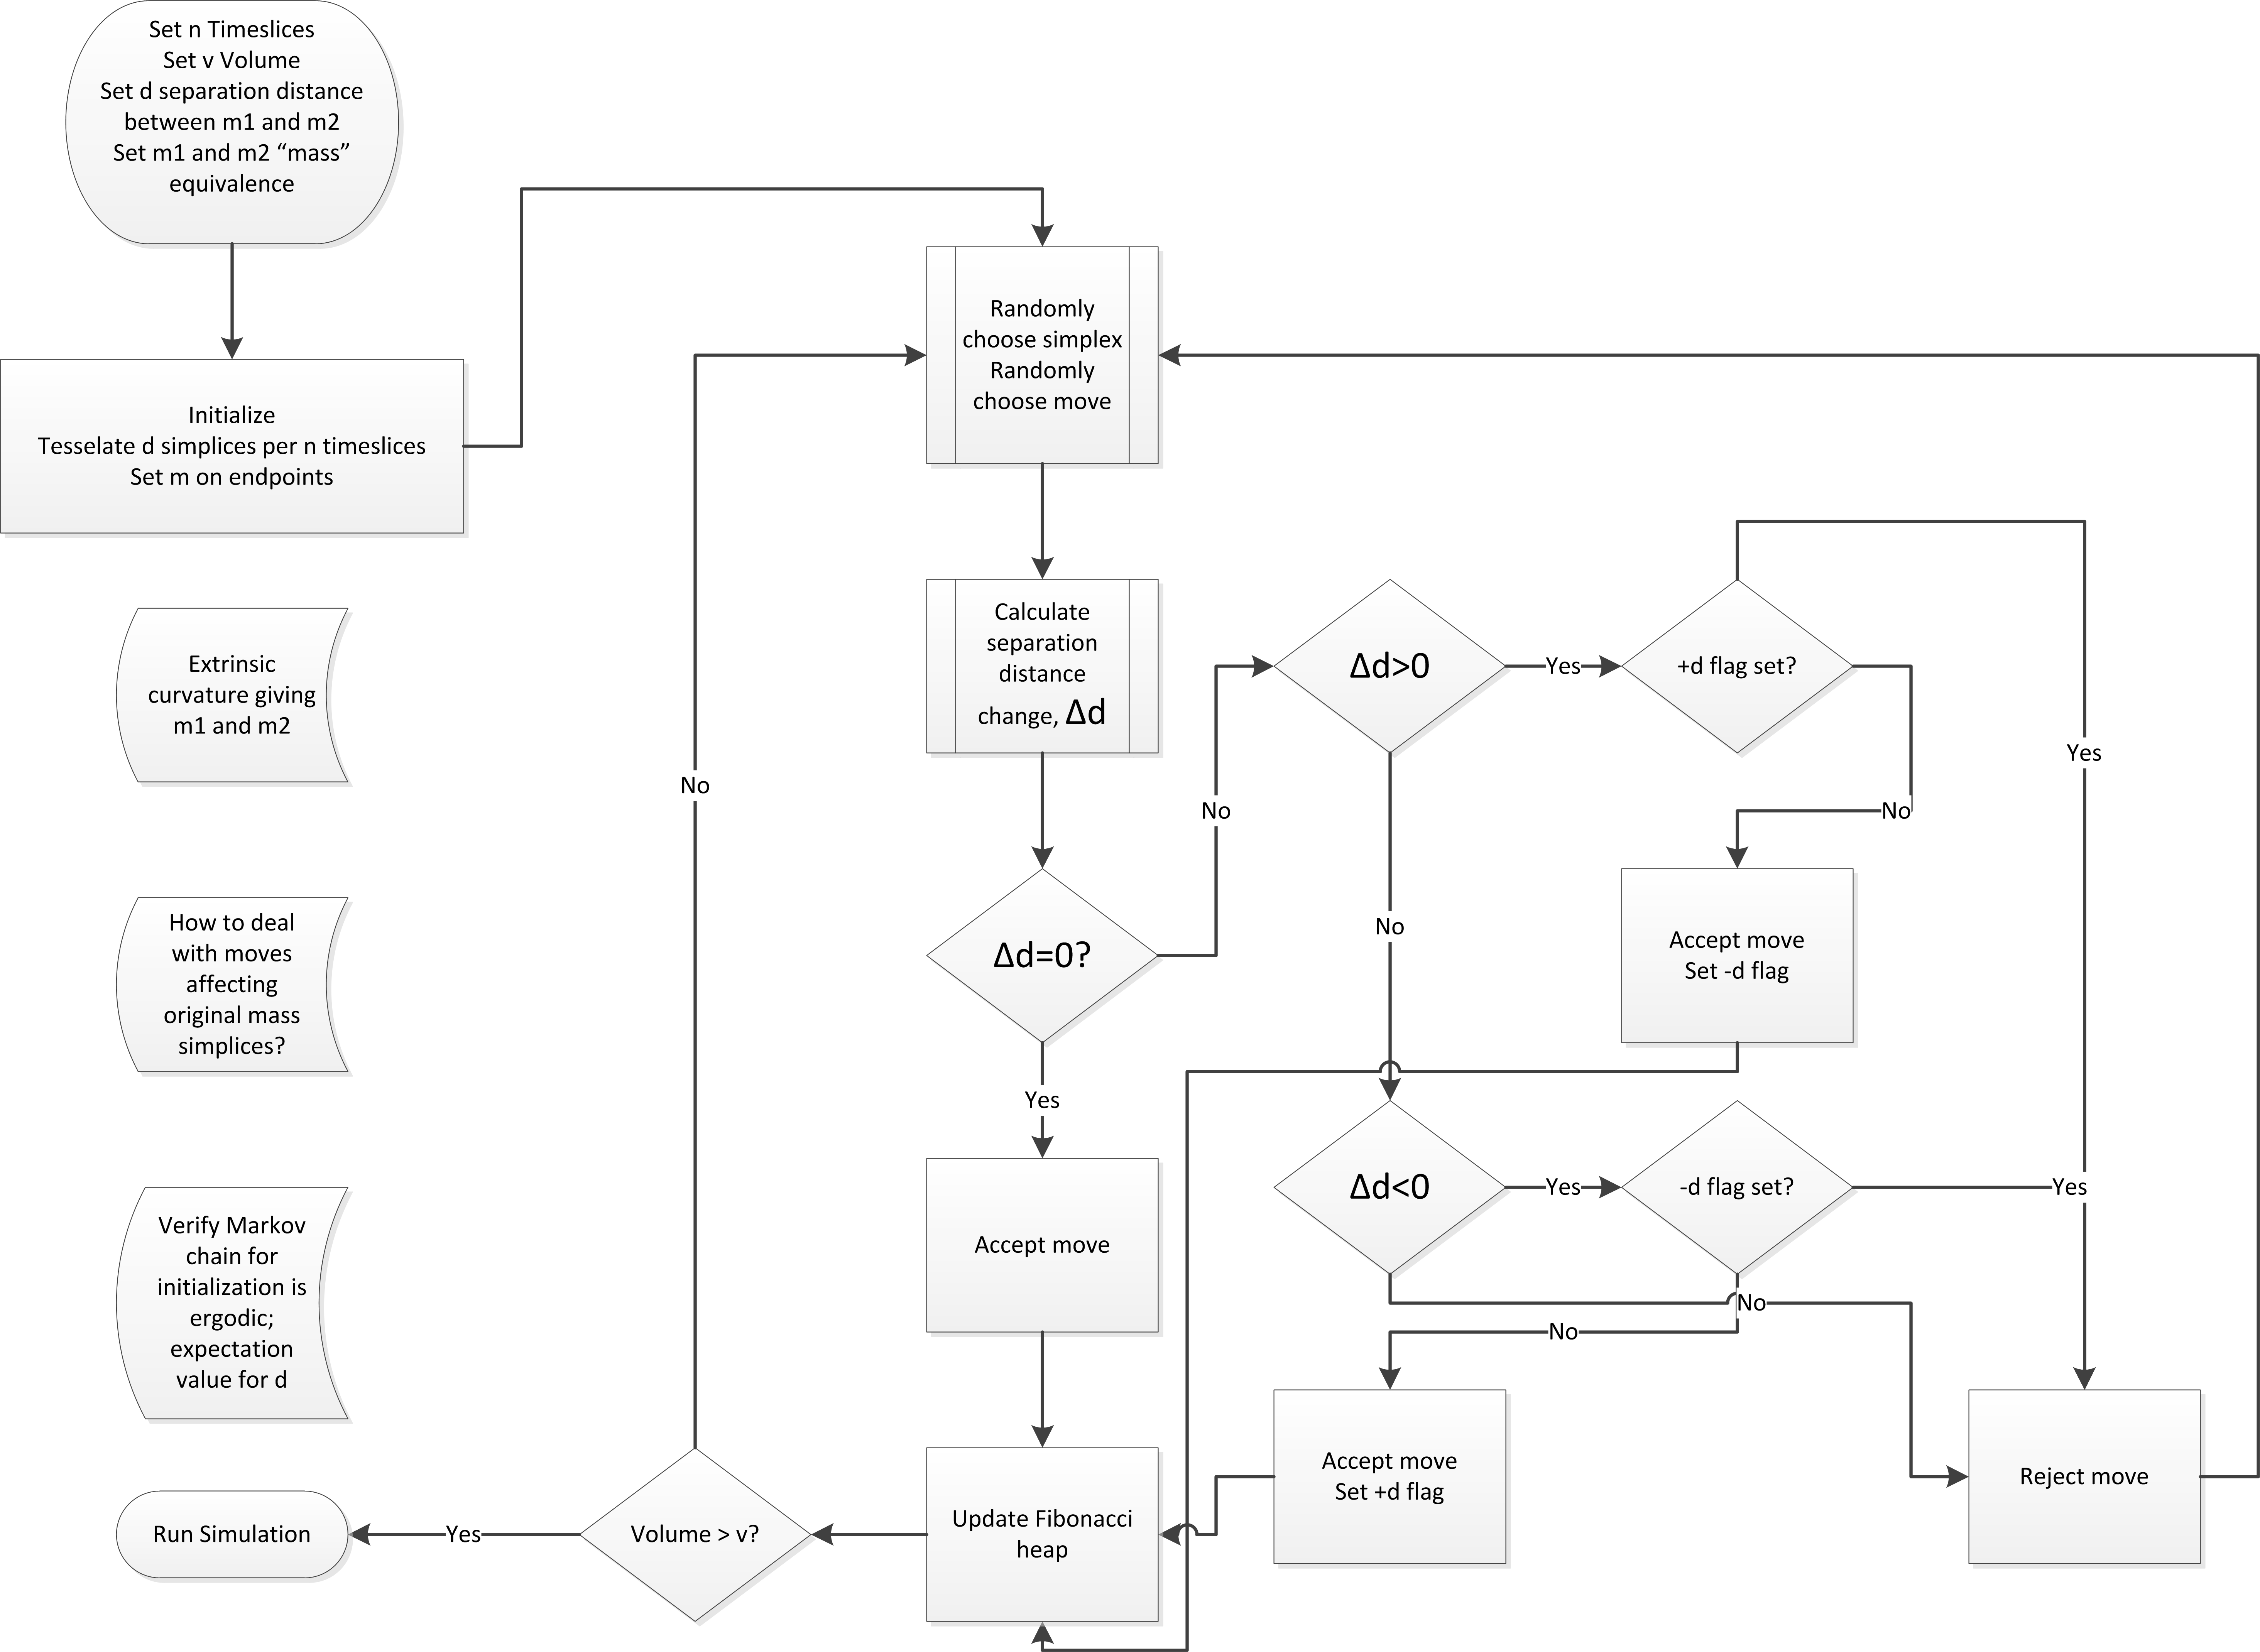
\includegraphics[scale=0.35]{Initialization}

Dijkstra's Algorithm \cite{cormen2001introduction}


Solves single-source shortest-path problems on weighted, directed
graph G=(V,E) of non-negative edge lengths

\begin{itemize}
\item Greedy algorithm
\item Proven to be correct
\item Complexity

\begin{itemize}
\item $O(V^{2})$ naively using adjacency list
\item $O(E\lg V)$ using priority queue iff all vertices reachable from
source
\item $O(V\lg V+E)$ using Fibonacci heap (more relaxation calls than extract-min
calls)
\end{itemize}
\item Issue: confine edge length algorithm to particular time-slice
\item Solution: Store Fibonacci heap of simplices per time-slice

\begin{itemize}
\item Each simplex has 5 neighbors, so more compact than adjacency matrix
\end{itemize}

\begin{itemize}
\item How to deal with moves affecting original ``mass'' simplices
\item How to create a 4d cylinder of height z=d
\item Verify Markov chain for initialization is ergodic
\item Calculate <d>
\end{itemize}
\end{itemize}

\section{Summary}
\begin{itemize}
\item Insert mass equivalence via extrinsic curvature
\item Insert strut by enforcing separation distance
\item Filter moves which alter separation distance via Markov chain
\item Outlook

\begin{itemize}
\item Write code!
\item Check Extrinsic Curvature
\item Compare results
\end{itemize}
\end{itemize}

\bibliographystyle{ieeetr}
\bibliography{cdt-newtonian-limit-biblio}


\end{document}
